
\subsection{Description of Base Excision Repair}

This is from my thesis

So far we have seen some applications of CCB, which are very close to the original inspiration of the calculus. If the principles behind CCB are of some general relevance, there should be other processes we can model using our calculus. A candidate for these might be biological processes. These are ultimately chemical reactions, but they are often viewed at a much higher level of abstraction then we have done so far. Typically, in such studies atoms would no longer play a r\^{o}le, but proteins and other macromolecules, consisting of thousands or more atoms are considered as entities. Typical examples are pathways, gene regulation, transcription, or DNA repair. One of the mechanisms for DNA repair is \emph{base excision repair} (BER). Specifically, BER is responsible for repairing small damages, where a single base pair in the DNA is not correct. Such damages can be inflicted by processes in the body or various external factors like radiation. Repair of such damages is important to prevent a degradation of the DNA information in the organism. There are various subtypes of BER, and various proteins involved in it. For our purposes, we look at the case that a uracil base has been incorporated in the DNA. Uracil is normally only found in RNA, whereas DNA consists of the four bases adenine (A), cytosine (C), guanine (G), and thymine (T).

Uracil-DNA glycosylase (UNG or UDG) is the protein responsible for removing uracil from DNA and making the position available for insertion of the correct base. The process has been extensively studied\footnote{A good overview is given in \cite{pmid25252105}. We use a highly simplified view here. For example, there is not a single UDG, but a family of UDGs all exhibiting slightly different behaviour.} and modelled in \cite{Koehler2014} and \cite{kappadna}. A description of the process on an abstract level is as follows: UDG can bind to any of the deoxyribose/phosphate groups forming the backbone strands of the DNA. From there it can ``walk'' along the chain to the next deoxyribose/phosphate group (that walk makes it much more likely to find a damage than if UDG would just randomly bind to and get off the DNA strand again). If the base attached to this group is uracil, UDG will bind to it and dissolve the bond from the uracil to the DNA. Uracil can then be released and UDG can either continue the search or get off the DNA strand. The correct base can take the place of the uracil.

\subsection{Modelling BER}

In order to model BER, we need the following components: deoxyribose/phosphate groups, the UDG, the uracil and the four other bases. The other bases will not take part in the reactions, but include them in our model in order to demonstrate the interaction we. The components are the following:
%
$$\begin{array}{lll}
DP & \bydef & (p3,p5,b,d).DP'\\
UDG & \bydef & (h;f).(e).UDG'\\
U & \bydef & (b;e).(u).U'\\
A & \bydef & (b;i).(a).A'\\
T & \bydef & (b;i).(t).T'\\
G & \bydef & (b;i).(g).G'\\
C & \bydef & (b;i).(c).C'\\
\end{array}$$
%
where processes $A$, $T$, $G$, $C$, and $U$ model the bases adenine (A), cytosine (C), guanine (G), thymine (T), and uracil (U) respectively. Process $UDG$ represents the Uracil-DNA glycosylase and $DP$ a deoxyribose/phosphate group. Here $d$, $e$, $i$, and $f$ are weak actions, all other actions, namely $p3$, $p5$, $h$, $b$, $u$, $a$, $t$, $g$, and $c$ are strong.

The synchronisation function for our system is as follows:
%
$$\begin{array}{ l c l l }
\gamma(p3,p5) & = & p & \\
\gamma(b,b) & = & bb &\\
\gamma(a,t) & = & at &  \\
\gamma(g,c) & = & gc & \\
\gamma(h,d) & = & hd & \\
\gamma(f,d) & = & fd & \\
\gamma(e,e) & = & ee & \\
\end{array}$$
%
\begin{figure}[h!]
\psfrag{UDG}{${\mathrm{UDG}}$}
\psfrag{sp1}{${\mathrm{DP_1}}$}
\psfrag{sp2}{${\mathrm{DP_2}}$}
\psfrag{sp3}{${\mathrm{DP_3}}$}
\psfrag{sp4}{${\mathrm{DP_4}}$}
\psfrag{sp5}{${\mathrm{DP_5}}$}
\psfrag{sp6}{${\mathrm{DP_6}}$}
\psfrag{A}{${\mathrm{A}}$}
\psfrag{T}{${\mathrm{T}}$}
\psfrag{C1}{${\mathrm{C_1}}$}
\psfrag{C2}{${\mathrm{C_2}}$}
\psfrag{G1}{${\mathrm{G_1}}$}
\psfrag{G2}{${\mathrm{G_2}}$}
\psfrag{U}{${\mathrm{U}}$}
\psfrag{hd}{$hd$}
\psfrag{fd}{$fd$}
  \centering
    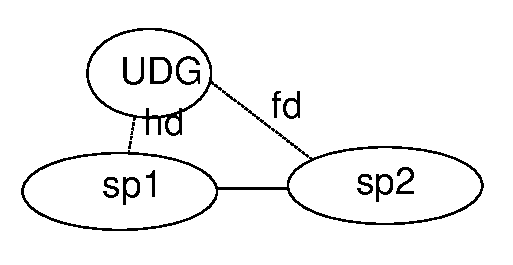
\includegraphics[width=1.0\textwidth]{ber/berintermediate}
  \caption[A $UDG$ unit whilst performing a step along a DNA strand.]{A $UDG$ unit whilst performing a step along a DNA strand. The $hd$ bond is broken together with the new $fd$ being formed.}
  \label{fig:berintermediate}
\end{figure}

We model the deoxyribose/phosphate groups first. This has two ends, normally called 3' and 5', which we model as $p3$ and $p5$ actions respectively. They help us to build the DNA strands. Also, there is a $b$ action, which enables binding of a base. Then we need a possibility for the UDG to bind and to ``walk'': this is enabled by actions $d$, $h$, and $f$, as we will see. UDG is modelled to have the prefix $(h;f)$, which enables the walk, since the strong action $h$ can be bonded to a $DP$ and $f$ can interact with a neighbouring $DP$. This breaks the $hd$ bond, and the $fd$ bond is then promoted to $d$, which gives us the $UDG$ being bonded to the neighbouring $DP$ the same way it was bound before to the other $DP$. Figure~\ref{fig:berintermediate} shows this intermediate situation whilst this step is performed. The five bases ($C$, $G$, $T$, $A$) all have a $b$ action to bind to a $DP$. If $A-T$ respectively $C-G$ are opposite each other they can bind and therefore form a correct base pair in the DNA. Uracil ($U$) is not able to form a base pair in our DNA context. All bases have a weak action in the prefix $(b;x)$. This action $x$ serves for removing the base from the DNA by breaking the $b$ bond. For uracil the action $x$ is $e$, for other bases it is $i$. By this UDG can be specific to uracil. In our model no action interacts with $i$, but of course other proteins not modelled might react with it. Note that $i$ and $e$ actions in the $U$, $A$, $T$, $G$, and $C$ processes cannot happen if the $u, a, t, g$ respctively $c$ actions are done, so $i$ and $e$ are blocked by $u, a, t, g,$ and $c$. Since $u, a, t, g$ and $c$ are used to form the base pairs this means that a correct base pair cannot be removed from the DNA in any case. This models the situation we need for the repair mechanism to work. We have used concerted actions in two instances here: Firstly to enable the UDG walk. This is an instance where backtracking would not work, since we need out-of-causal-order reversibility in this case. We cannot unbond from the old DP first and then choose the next $DP$, but we must hold the old bond until the new bond is formed. Secondly, we use a concerted action to enable the repair mechanism by making a bonding on the repair action break the bond to DP.

In the synchronisation function, we have the interaction of $p3$ and $p5$ to form the strands, the $b$-$b$ interaction for binding the bases, the $h$-$d$ and $f$-$d$ interaction for the ``walk'', the $a$-$t$ and $g$-$c$ interactions for forming the base pairs, and the $e$-$e$ interaction for the repair action.

In order to model a strand of DNA, we restrict ourselves to three base pairs. This means we need six $DP$ processes and six bases. We put two ``correct'' base pairs and one containing a uracil base. An extra $C$ base must be available for replacing $U$. We also use subscripts to distinguish processes where there is more than one instance of the process. The system is modelled in CCB as follows:

$$\begin{array}{l}
(DP_1 \paral DP_2 \paral DP_3 \paral A \paral T \paral G_1 \paral G_2 \paral U \paral C_1 \paral C_2 \paral DP_4 \paral DP_5 \paral DP_6 \paral UDG) \\
\setminus\{p3, p5, d, b, a, t, g, e, u, c, h, f, i\} 
\end{array}$$ 

We leave out the restriction from now on for ease of reading. We number actions using subscripts where there is more than one instance, and set initial bonds as required. We get the following process:
%
\begin{flalign*}
&(p3_1,p5_1[1],d_1,b_1[5]).DP_1' \paral (p3_2[1],p5_2[3],d_2,b_2[4]).DP_2' \paral (p3_3[3],p5_3,d_3,b_3[9]).DP_3' \paral &&\\
&(b_1[5];i_1).(a[6]).A' \paral (b_2[7];i_2).(t[6]).T' \paral (b_3[8];i_3).(g_1).G_1' \paral  ((b_4[9];i_4).(g_2[10]).G_2'  \paral &&\\
&(b_5[4];e_2).(u).U' \paral (b_6[11];i_6).(c_1[10]).C' \paral (b_7;i_7).(c_2).C' \paral (p3_4,p5_4[12],d_4,b_4[7]).DP_4' \paral &&\\ &(p3_5[12],p5_5[13],d_5,b_5[8]).DP_5' \paral (p3_6[13],p5_6,d_6,b_6[11]).DP_6' \paral (h;f).(e_2).UDG'&&
\end{flalign*}
%
\begin{figure}[h!]
\psfrag{UDG}{${\mathrm{UDG}}$}
\psfrag{sp1}{${\mathrm{DP_1}}$}
\psfrag{sp2}{${\mathrm{DP_2}}$}
\psfrag{sp3}{${\mathrm{DP_3}}$}
\psfrag{sp4}{${\mathrm{DP_4}}$}
\psfrag{sp5}{${\mathrm{DP_5}}$}
\psfrag{sp6}{${\mathrm{DP_6}}$}
\psfrag{A}{${\mathrm{A}}$}
\psfrag{T}{${\mathrm{T}}$}
\psfrag{C1}{${\mathrm{C_1}}$}
\psfrag{C2}{${\mathrm{C_2}}$}
\psfrag{G1}{${\mathrm{G_1}}$}
\psfrag{G2}{${\mathrm{G_2}}$}
\psfrag{U}{${\mathrm{U}}$}
\psfrag{1}{${\mathrm{1}}$}
\psfrag{2}{${\mathrm{2}}$}
  \centering
    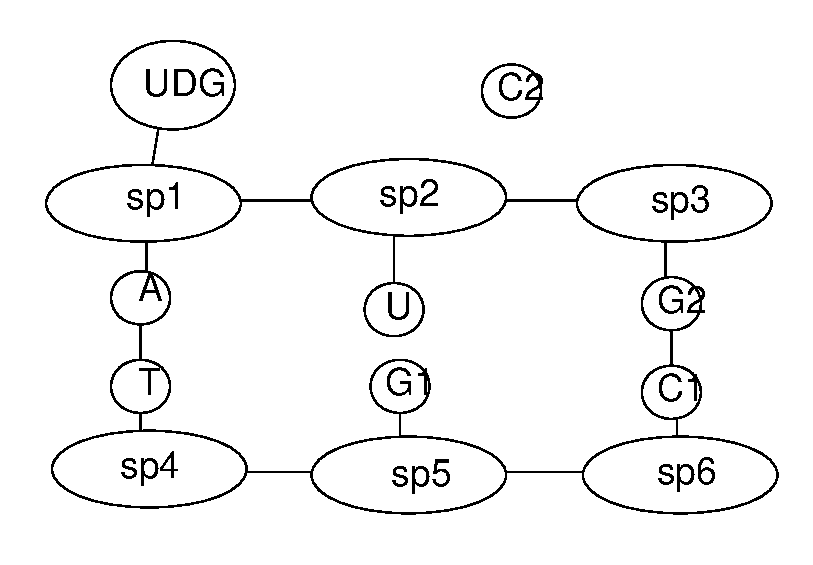
\includegraphics[width=1.0\textwidth]{ber/ber}
  \caption[A three base pair DNA fragment.]{A three base pair DNA fragment, with a uracil instead of a cytosine, and a UDG protein attached.}
  \label{fig:ber}
\end{figure}

Initially $UDG$ bonds to $DP_1$, which in turn is bonded to a correct base pair (note $UDG$ was not bound so far to any other process). The situation is shown in Figure~\ref{fig:ber} and is as follows (the bonds created, news keys and action on which keys were removed are shown in \textbf{bold}):
%
\begin{flalign*}
&\xrightarrow{hd[2]}(p3_1,p5_1[1],d_1\boldsymbol{[2]},b_1[5]).DP_1' \paral (p3_2[1],p5_2[3],d_2,b_2[4]).DP_2' \paral &&\\
&(p3_3[3],p5_3,d_3,b_3[9]).DP_3' \paral
(b_1[5];i_1).(a[6]).A' \paral (b_2[7];i_2).(t[6]).T' \paral (b_3[8];i_3).(g_1).G_1' \paral &&\\
&((b_4[9];i_4).(g_2[10]).G_2'  \paral (b_5[4];e_2).(u).U' \paral (b_6[11];i_6).(c_1[10]).C' \paral (b_7;i_7).(c_2).C' \paral &&\\
&(p3_4,p5_4[12],d_4,b_4[7]).DP_4' \paral (p3_5[12],p5_5[13],d_5,b_5[8]).DP_5' \paral &&\\
&(p3_6[13],p5_6,d_6,b_6[11]).DP_6' \paral (h\boldsymbol{[2]};f).(e_2).UDG'&&
\end{flalign*}
%
The UDG can now randomly ``walk'' along the chain. The $(h;f)$ prefix can appropriately model this, since if the weak $f$ action binds to the neighbour, the bond on $h$ is broken. In our case, action $f$ in $UDG$ can communicate with $d_2$ in $DP_2$. This breaks bond 2 from $h$ in $UDG$ to $d_1$ in $DP_1$, thus having performed a ``step''. We then move key $14$ from $f$ to $h$ (via the \rulename{prom} rule from Figure~\ref{fig:reduction}) and get:
%
\begin{flalign*}
&\xrightarrow{\{fd[14],\underline{hd}[2]\}} \Rightarrow (p3_1,p5_1[1],\boldsymbol{d_1},b_1[5]).DP_1' \paral (p3_2[1],p5_2[3],\boldsymbol{d_2[14]},b_2[4]).DP_2' \paral&&\\
&(p3_3[3],p5_3,d_3,b_3[9]).DP_3' \paral (b_1[5];i_1).(a[6]).A' \paral (b_2[7];i_2).(t[6]).T' \paral (b_3[8];i_3).(g_1).G_1' \paral&&\\
&((b_4[9];i_4).(g_2[10]).G_2'  \paral (b_5[4];e_2).(u).U' \paral (b_6[11];i_6).(c_1[10]).C' \paral (b_7;i_7).(c_2).C' \paral&&\\
&(p3_4,p5_4[12],d_4,b_4[7]).DP_4' \paral (p3_5[12],p5_5[13],d_5,b_5[8]).DP_5' \paral\\ &(p3_6[13],p5_6,d_6,b_6[11]).DP_6' \paral \boldsymbol{(h[14];f)}.(e_2).UDG'&&
\end{flalign*}
%
$UDG$ could now simply continue its walk, or it can interact via its $e$ action with the uracil. Note that other bases expose the $i$ action, so uracil cannot interact with them. The $u$, $a$, $t$, $g$, or $ c$ actions block $e$ or $i$, so correct base pairs are not affected by repairs. In our example $e_2$ on $UDG$ interacts with $e_2$ on $U$, breaking bond 4 between $b_5$ in $UDG$ and $b_2$ in $DP_2$. We have achieved the desired repair, since the uracil is removed from the DNA. We model this by the following transition (we use the rewrite rule again):
%
\begin{flalign*}
&\xrightarrow{\{ee[15],\underline{bb}[4]\}} \Rightarrow (p3_1,p5_1[1],d_1,b_1[5]).DP_1' \paral (p3_2[1],p5_2[3],d_2[14],\boldsymbol{b_2}).DP_2' \paral&&\\
&(p3_3[3],p5_3,d_3,b_3[9]).DP_3' \paral (b_1[5];i_1).(a[6]).A' \paral (b_2[7];i_2).(t[6]).T' \paral (b_3[8];i_3).(g_1).G_1' \paral&&\\
&((b_4[9];i_4).(g_2[10]).G_2'  \paral \boldsymbol{(b_5[15];e_2)}.(u).U' \paral (b_6[11];i_6).(c_1[10]).C' \paral (b_7;i_7).(c_2).C' \paral&&\\
&(p3_4,p5_4[12],d_4,b_4[7]).DP_4' \paral (p3_5[12],p5_5[13],d_5,b_5[8]).DP_5' \paral\\ &(p3_6[13],p5_6,d_6,b_6[11]).DP_6' \paral (h[14];f).(\boldsymbol{e_2[15]}).UDG'&&
\end{flalign*}
%
The floating $C_2$ can now take the place of the $U$ by binding to $DP_2$ and $G_1$. This is represented by the following two transitions:
%
\begin{flalign*}
&\xrightarrow{bb[16]}\xrightarrow{gc[17]}(p3_1,p5_1[1],d_1,b_1[5]).DP_1' \paral (p3_2[1],p5_2[3],d_2[14],\boldsymbol{b_2[16]}).DP_2' \paral&&\\
&(p3_3[3],p5_3,d_3,b_3[9]).DP_3' \paral (b_1[5];i_1).(a[6]).A' \paral (b_2[7];i_2).(t[6]).T' \paral (b_3[8];i_3).(\boldsymbol{g_1[17]}).G_1' \paral&&\\
&((b_4[9];i_4).(g_2[10]).G_2'  \paral (b_5[15];e_2).(u).U' \paral (b_6[11];i_6).(c_1[10]).C' \paral (\boldsymbol{b_7[16]};i_7).(\boldsymbol{c_2[17]}).C' \paral&&\\
&(p3_4,p5_4[12],d_4,b_4[7]).DP_4' \paral (p3_5[12],p5_5[13],d_5,b_5[8]).DP_5' \paral\\ &(p3_6[13],p5_6,d_6,b_6[11]).DP_6' \paral (h[14];f).(e_2[15]).UDG'&&
\end{flalign*}
%
The resulting process is shown in Figure~\ref{fig:ber2}.

\begin{figure}[h!]
\psfrag{UDG}{${\mathrm{UDG}}$}
\psfrag{sp1}{${\mathrm{DP_1}}$}
\psfrag{sp2}{${\mathrm{DP_2}}$}
\psfrag{sp3}{${\mathrm{DP_3}}$}
\psfrag{sp4}{${\mathrm{DP_4}}$}
\psfrag{sp5}{${\mathrm{DP_5}}$}
\psfrag{sp6}{${\mathrm{DP_6}}$}
\psfrag{A}{${\mathrm{A}}$}
\psfrag{T}{${\mathrm{T}}$}
\psfrag{C1}{${\mathrm{C_1}}$}
\psfrag{C2}{${\mathrm{C_2}}$}
\psfrag{G1}{${\mathrm{G_1}}$}
\psfrag{G2}{${\mathrm{G_2}}$}
\psfrag{U}{${\mathrm{U}}$}
\psfrag{1}{${\mathrm{1}}$}
\psfrag{2}{${\mathrm{2}}$}
  \centering
    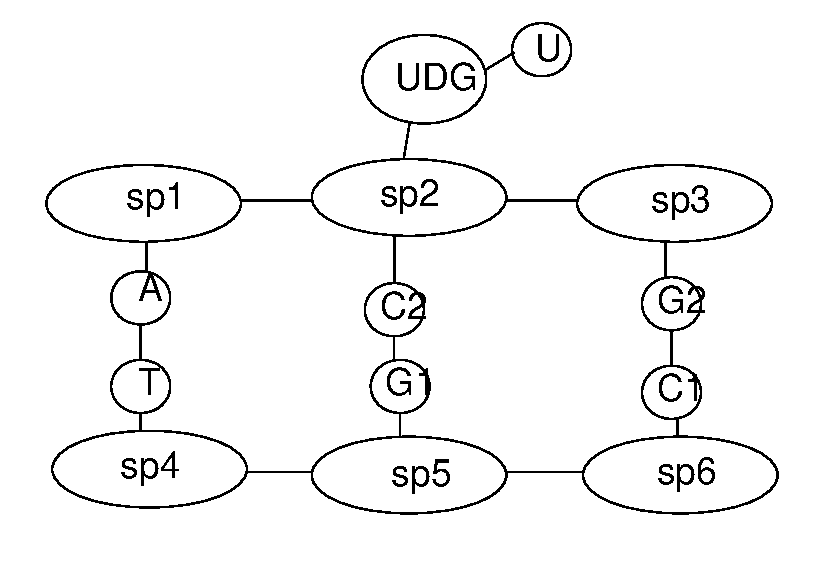
\includegraphics[width=1.0\textwidth]{ber/ber2}
  \caption[The repaired DNA fragment.]{The repaired DNA fragment, with the uracil replaced by a cytosine.}
  \label{fig:ber2}
\end{figure}

If uracil would have been bonded on $u$, the interaction with UDG could not have happened, so the defect is recognized. We now have the uracil broken from the deoxyribose/phosphate group and the $b$ action on the deoxyribose/phosphate group ready to bond to another base. UDG needs to release $U$ and then either to continue its walk or release itself from the DNA. We can again use our new operator for modelling UDG, since this way we achieve that the repair mechanism happens. On the other hand by combining two groups of actions we ``block'' this repair to happen if the desired second bond is there.

A limitation of our modelling is that it allows the UDG during its ``walk'' to bind to any DG group, since there is no restriction which $d$ action is used. In reality of course UDG must continue with the nearest DP group. This is a spatial effect our calculus does not model so far. Similarly, the repair by UDG binding to the $e$ action of a uracil (U) is not dependent on the UDG being next to it, whereas in reality it is. Again this is a spatial effect, which we will discuss in Section~\ref{sec:ccbs}.

We have used the software from Chapter~\ref{sec:simulation} to test the modelling. The desired path is one of the possibilities, which shows that our modelling is adequate in this respect. We also get some undesired reactions: Apart from UDG binding to any DP group during its walk, there is also the possibility that the unused $p5$ action of a $DP$, which is at the end of the DNA strand, interacts with an unused $p3$ from the a DP at the other end of the DNA strand. This is not impossible as a such, but prevented in reality by at least two effects we do not model. One is again the spatial arrangement, the other is the fact that the ends of the DNA are protected by special groups, which we do not model here. They prevent reactions at the DNA ends.
